\documentclass[conference]{IEEEtran}
\IEEEoverridecommandlockouts

% Packages
\usepackage{cite}
\usepackage{amsmath,amsfonts}
\usepackage{algorithm}
\usepackage{algpseudocode}
\usepackage{graphicx}
\usepackage{textcomp}
\usepackage{xcolor}
\usepackage{booktabs}
\usepackage{adjustbox}
\usepackage{listings}

\usepackage{verbatim}
\usepackage{multirow}

\def\BibTeX{{\rm B\kern-.05em{\sc i\kern-.025em b}\kern-.08em
    T\kern-.1667em\lower.7ex\hbox{E}\kern-.125emX}}

\begin{document}

\title{Deliverable report \\
\footnotesize \textit{"Diego Oniarti": Mat: 257835, \texttt{diego.oniarti@studenti.unitn.it}, GitRepo: \texttt{https://github.com/diego-oniarti/GPU\_homework}}}

\maketitle

\begin{abstract}
[max 200 words]\\
The sparse matrix-dense vector multiplication (SpMV) is a common linear algebra operation involving a sparse matrix and a dense vector. SpMV is widely used in many real-world applications such as \dots

This deliverable discusses \dots
\end{abstract}

\begin{IEEEkeywords}
Sparse Matrix, SpMV, CUDA, Parallelization, Storage Format
\end{IEEEkeywords}

\section{Introduction}
[max 300 words]\\
Introduce SpMV application and its parallelization challenges \dots

\section{Problem Statement}
Define the problem statement, including a description of the storage format used and a brief discussion of the parallelization approach (e.g., using CUDA).

\subsection{Storage Format}
Details about the format (e.g., CSR, COO, etc.) \dots

\subsection{Parallelization}
Describe the CUDA implementation approach \dots

\section{State of the Art}
Describe the available library solutions for the SpMV problem, including references and citations \cite{asimov1950irobot, svevo1923coscienza, pirandello1926uno}.

\section{Methodology and Contributions}\label{sec:methodology}

Describe the methodology used during the analysis, the compared algorithms and the expected outcomes. Use pseudo-codes like Algorithm \ref{alg:COOaggr} to describe your own implemented kernels.

\noindent Include at least the following implementations:
\begin{itemize}
    \item Naive CPU implementation
    \item Optimised CPU implementation based on cache behaviour
    \item GPU naive implementation
\end{itemize}

\noindent For the analysis include
\begin{itemize}
    \item Valgrind and runtime comparison between the CPU implementations 
    \item Runtime CPU vs GPU comparison looping over different matrix dimensions
\end{itemize}

\begin{algorithm}[h!]
\caption{Algorithm for the vector addition}
\algorithmicrequire~The input vectors $a$ and $b$ of size $nnz$.
\begin{algorithmic}[1]
\Procedure{Function}{$a$, $b$, $nnz$}
\State $c \gets \emptyset$\label{partitioning}
\For{$i$ in $\{1 \dots nnz\}$ \textbf{parallel}}
\State $c[i] = a[i] + b[i]$\label{partitioning}
\EndFor
\State \textbf{return} $c$\Comment{the result vector}
\EndProcedure
\end{algorithmic}
\label{alg:COOaggr}
\end{algorithm}

\section{System Description and Experimental Set-up}

Use this section to describe system, dataset and experimental set-up.

\subsection{System Description}

Describe the used system and the software environment (CUDA version, GCC version, \dots). Decide which information are valuable to group into a table like Table \ref{tab:system_description} and which are more valuable to be described in the text.

\begin{table}[ht]
    \centering
    \begin{adjustbox}{width=\columnwidth}
    \begin{tabular}{lllrl}
    \toprule
    \textbf{System} &  \textbf{Processor} & \textbf{Cores per Socket} & \textbf{RAM} & \textbf{Accelerator} \\
    \midrule
    Leonardo &  Intel Xeon 8358 CPU & 32 at 2.6 GHz & 494 GB & NVIDIA A100 \\
    Local &  2$\times$ AMD Rome 7742 & 64 at 2.25 GHz & 1,007 GB & NVIDIA A100 \\
    \bottomrule
    \end{tabular}
    \end{adjustbox}
    \vspace{1em}
    
    \caption{System details}
    \label{tab:system_description}
\end{table}

\subsection{Dataset description}

Discribe the used dataset and the reasons of your choice. List the used input matrices and all the information that you think are valuable to show (number of non-zero elements, sparsity ratio, \dots); Table \ref{tab:my_label} gives you a possible example.

\begin{table}[]
    \centering
    \begin{adjustbox}{width=\columnwidth}
    \begin{tabular}{lrrrrc}
    \toprule
    \textbf{Dataset} & \multicolumn{1}{c}{$\mathbf{|V|}$} & \multicolumn{1}{c}{$\mathbf{|E|}$} & \multicolumn{1}{c}{\textbf{Avg. Degree}} & \textbf{Diameter} & \textbf{Benchmark} \\
    \midrule
    com-youtube \cite{snapnets} & 1,134,890 & 2,987,624 & 5.27 & 20 & \multirow{5}{*}{\shortstack[t]{Naive vs optimized CPU}}\\
    amazon-ratings \cite{rossi2015network}& 2,146,057 & 5,743,146 & 5.35 & 28& \\
    cit-patents \cite{rossi2015network} & 3,764,117 & 16,511,741 & 8.77 & 26&\\
    com-lj \cite{rossi2015network}&3,997,962 & 34,681,189 &17.35 &17 &\\
    dblp \cite{rossi2015network}& 4,000,148 & 8,649,011 &4.32 &50 &\\
    \midrule
    flickr-link \cite{alghamdi2017benchmark} &1,624,992&15,472,576&19.04&24 &\multirow{4}{*}{\shortstack[c]{CPU vs GPU}} \\
    Wiki-Talk \cite{alghamdi2017benchmark} & 2,388,953&4,656,682&3.90&9 &\\
    com-Orkut \cite{snapnets} &3,072,441&117,185,083&76.28&9 &\\
    dbpedia-link \cite{alghamdi2017benchmark} &18,265,512&126,888,089&13.98&12 &\\
    \bottomrule
    \end{tabular}
    \end{adjustbox}
    \vspace{1em}
    
    \caption{Caption}
    \label{tab:my_label}
\end{table}

\subsection{Experimental Set-up}
Explain the benchmark metrics and all the experimental set-up (warm-up cycles, number of performed runs\dots).

\section{Experimental Results}
Present and discuss results. Include plots and tables when required (like Figure \ref{fig:enter-label}). Do not simply describe the figures; criticise the achieved results by underlining how they confirm/differ from the expected outcomes described in Section \ref{sec:methodology}.

\begin{figure}
    \centering
    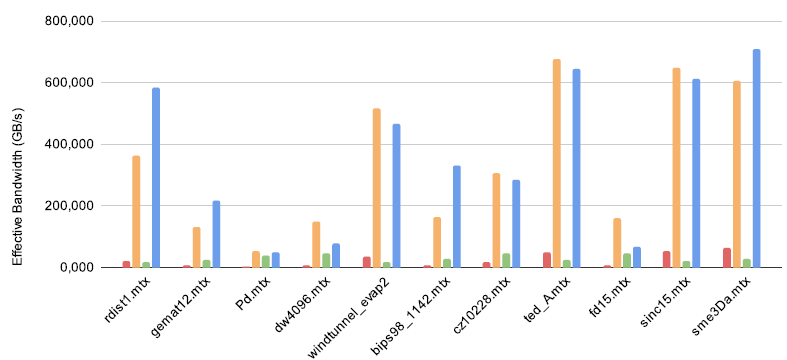
\includegraphics[width=0.95\linewidth]{SampleImage.png}
    \caption{Caption}
    \label{fig:enter-label}
\end{figure}

\section{Conclusions}
[max 200 words]\\
Summarize findings and future work \dots

\bibliographystyle{IEEEtran}
\bibliography{references}

\end{document}

